

\subsection{1.29 Карбонильные комплексы переходных металлов. Способы получения и условия стабильности, геометрия, электронное строение,свойства. Сравнение карбонилов различных металлов между собой.}
\textbf{Получение}\\
\begin{itemize}
	\item Металл $+ CO$:
	\[
	Ni + 4CO = Ni(CO)_4
	\]
	\item Соль металла + восстановитель + $CO$:
	\[
	CrCl_3 + Al + 6CO = AlCl_3 = Cr(CO)_6 + AlCl_3
	\]
	\item Экзотика: 
	\[
	2Fe(CO)_5 = h\nu = Fe_2(CO)_9 + CO
	\]
\end{itemize}
\textbf{Условия стабильности}\\
Правило 18 электронов \\
\textbf{Геометрия}\\
\begin{figure} [H]
	\centering {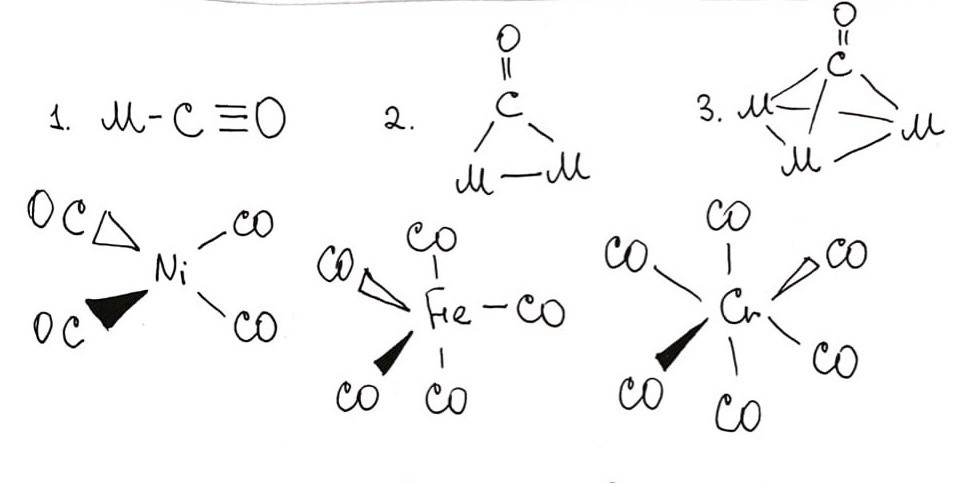
\includegraphics[scale=0.4]{dd2}}
\end{figure}
\begin{itemize}
	\item Различные полиэдры
	\item Возможно с мостиковыми лигандами и связями $M-M$
\end{itemize}
\begin{figure} [H]
	\centering {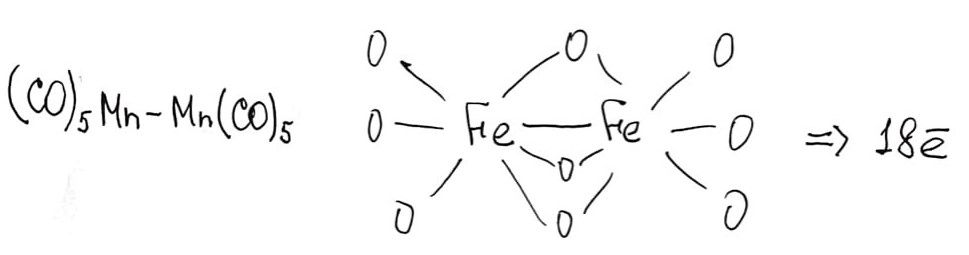
\includegraphics[scale=0.4]{dd3}}
\end{figure}
Чем ниже по группе, тем меньше вероятность мостиков. \\
\textbf{Электронное строение}\\
$\left[ M-C\equiv O \leftrightarrow M = C = O ) \right]$ \\
\begin{figure} [H]
	\centering {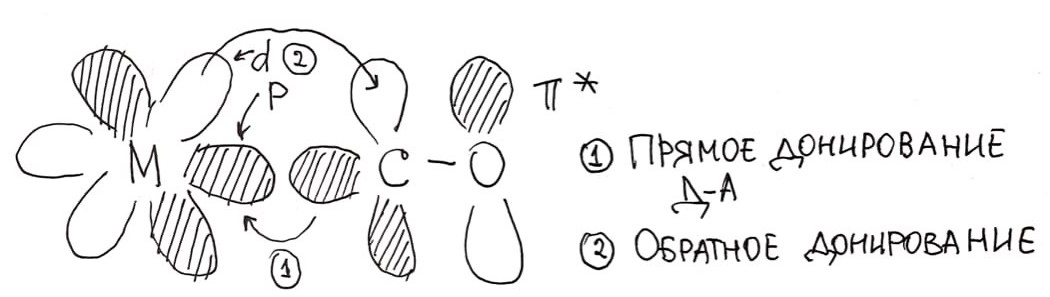
\includegraphics[scale=0.4]{dd4}}
\end{figure}
\textbf{Свойства}\\
\begin{itemize}
	\item Замещение
	\[
	Cr(CO)_6 + NR_3 = P_3NCr(CO)_5 + CO
	\]
	\item $\rightarrow $ анион
	\[
	Fe(CO)_5 = Na/Hg = Na_2^{+} \left[Fe(CO)_4 \right]^{2-}
 	\]
	\item $Nu$-атака по $CO$
	\[
	Fe(CO)_5 + NaOH = Na \left[ HFe(CO)_4 \right]
	\]
\end{itemize}
\textbf{Сравнение}\\
У $Sc$ и $Cu$ нет карбонильных комплексов, т.к. $d$-орбиталь лежит слишком высоко/слишком низко по энергии, $Ti(CO)_7$ не существует из-за стерического эффекта, у $V(CO)_6$ - $17$ электронов, у $Mn, Co$ - димеры ($Mn_2(CO)_{10}, Co_2(CO)_8$) 


